\documentclass[a4paper]{scrartcl}

\usepackage[a4paper, total={6in, 8in}]{geometry}

\usepackage{pdfpages} 

\usepackage{minted}

\title{COL216 Assignment 2\\{\Large Stage 1}}
\date{9 February 2022}
\author{Rishabh Dhiman\\ \texttt{2020CS10837}}

\usepackage{amsthm, amsmath, amssymb}
\usepackage{hyperref}

\theoremstyle{definition}
\newtheorem{definition}{Definition}

\renewcommand{\tt}{\mintinline{text}}
\newcommand{\fun}{\mintinline{cpp}}
\newcommand{\reg}{\mintinline{text}}

\begin{document}

\maketitle

\section{Objective}
Construct an ALU, a register file, a primary memory unit and a data memory unit for an ARM processor in VHDL.

\section{Technical Details}
\begin{itemize}
	\item The VHDL code was compiled and simulated using GHDL 1.0.0.
	\item The waveform viewer used is GTKWave Analyzer v3.3.104.
\end{itemize}

\section{Documentation}
The submission contains four VHDL files defining the units,
\begin{itemize}
	\item \tt{types.vhdl},
	\item \tt{alu.vhdl},
	\item \tt{reg_file.vhdl}, and
	\item \tt{memory.vhdl}.
\end{itemize}
Along with four testbenches for testing these units
\begin{itemize}
	\item \tt{alu_testbench.vhdl},
	\item \tt{reg_file_testbench.vhdl},
	\item \tt{primary_memory_testbench.vhdl}, and
	\item \tt{data_memory_testbench.vhdl}.
\end{itemize}

Along with an output folder, containing the waveforms on simulating the testbenches, in the form of .ghw and .pdf files.

\subsection*{\tt{types.vhdl}}
This files defines some custom types for words, half-words and bytes along with an enumerated type for opcodes. It's taken from Piazza post 163.

\subsection*{\tt{alu.vhdl}}
It defines the ALU satisfying the specifications given in the problem statement.

\subsection*{\tt{reg_file.vhdl}}
It defines the register file satisfying the specifications given in the problem statement.

\subsection*{\tt{memory.vhdl}}
It defines the primary memory and data memory satisfying the specifications given in the problem statement.

Since the contents primary memory had to be defined in the declaration itself, I decided to define it such that the entire memory contains $0$, barring the index $1$ which contains 0x0000FFFF.

\section{Tests and Results}
It was simulated using ghdl, the waveform was generated only till at most time 2500ns.

The output waveform of the testbench results can be viewed in .ghw and .pdf files.

The .pdf files don't contain the entire waveform due to a lack of space, however, the .ghw files can be opened in any waveform analyzer like GTKWave to view the output waveform.

The pdf files are also attached at the end of this report.

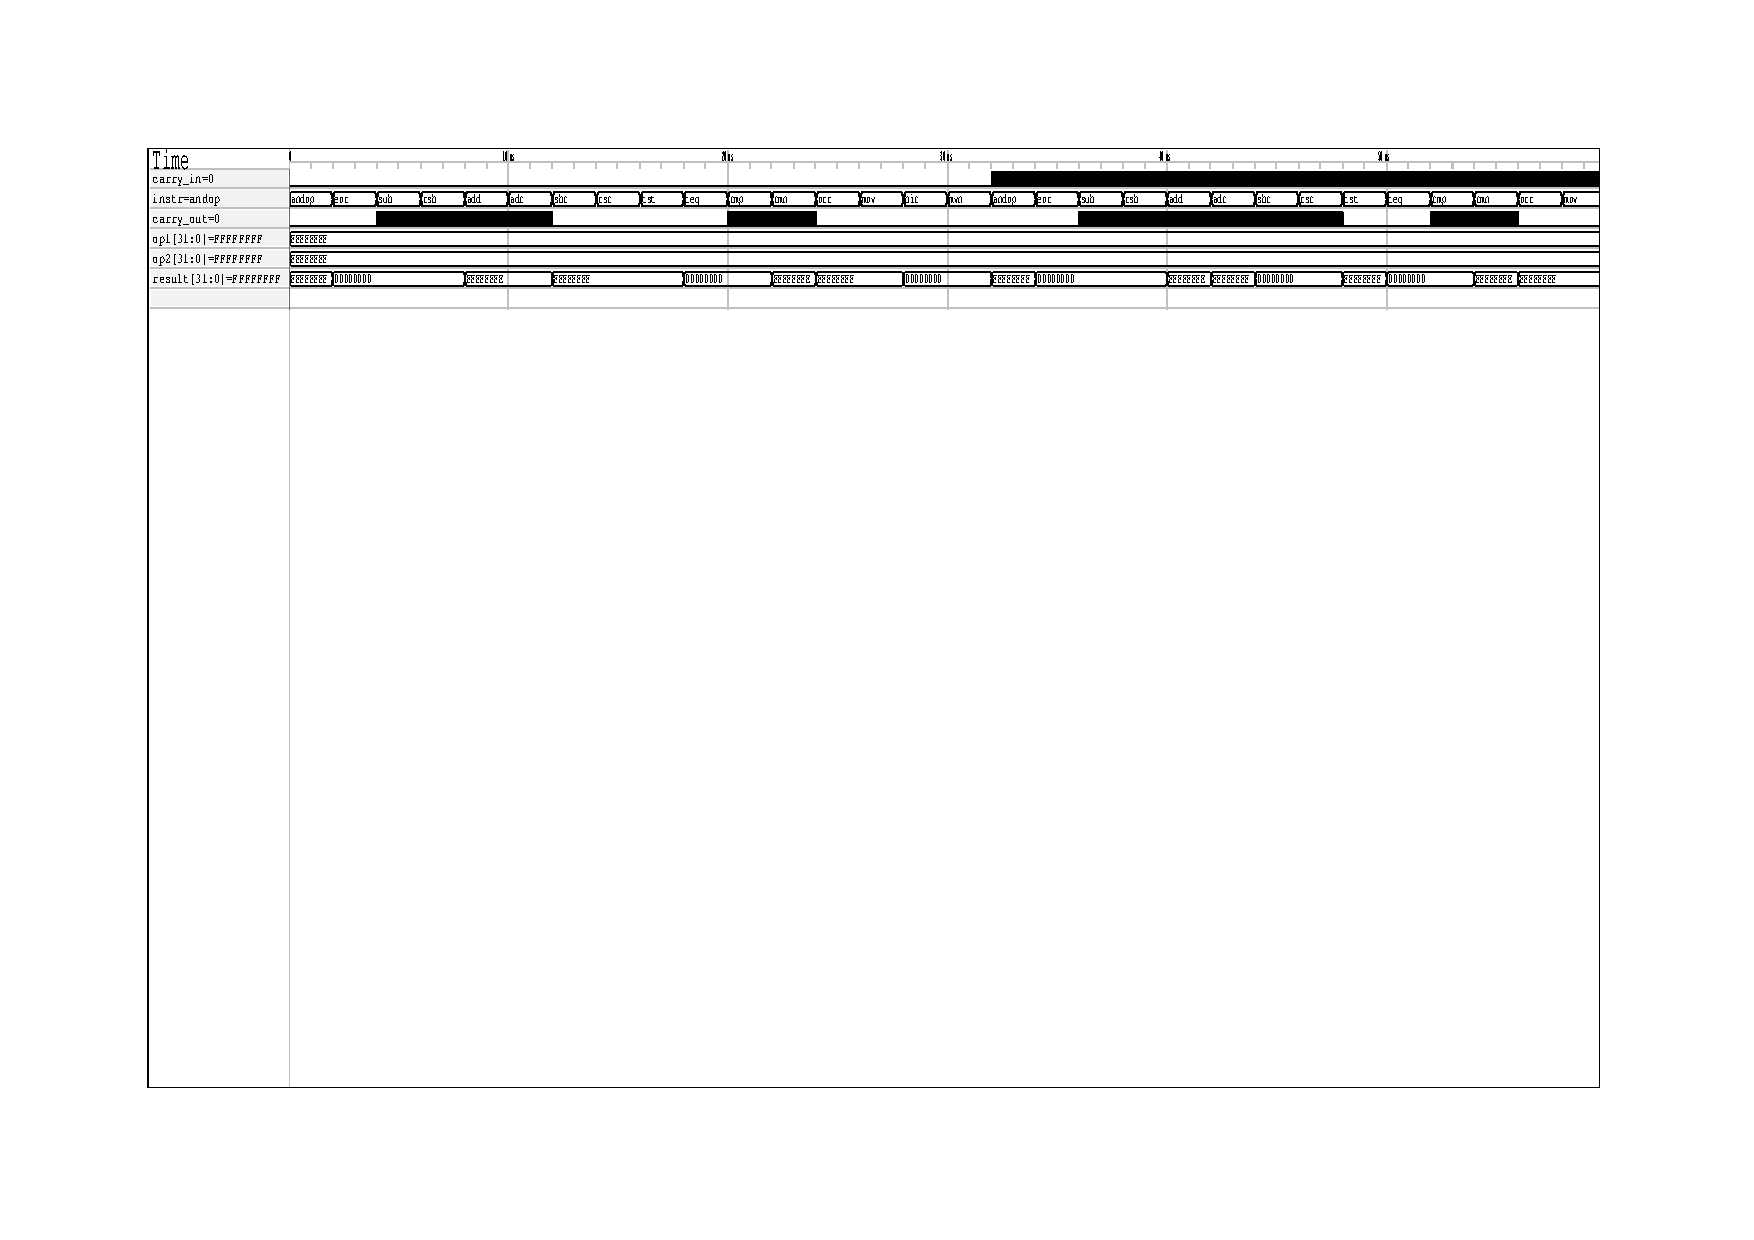
\includepdf[landscape=true]{../output/alu_tb.pdf}
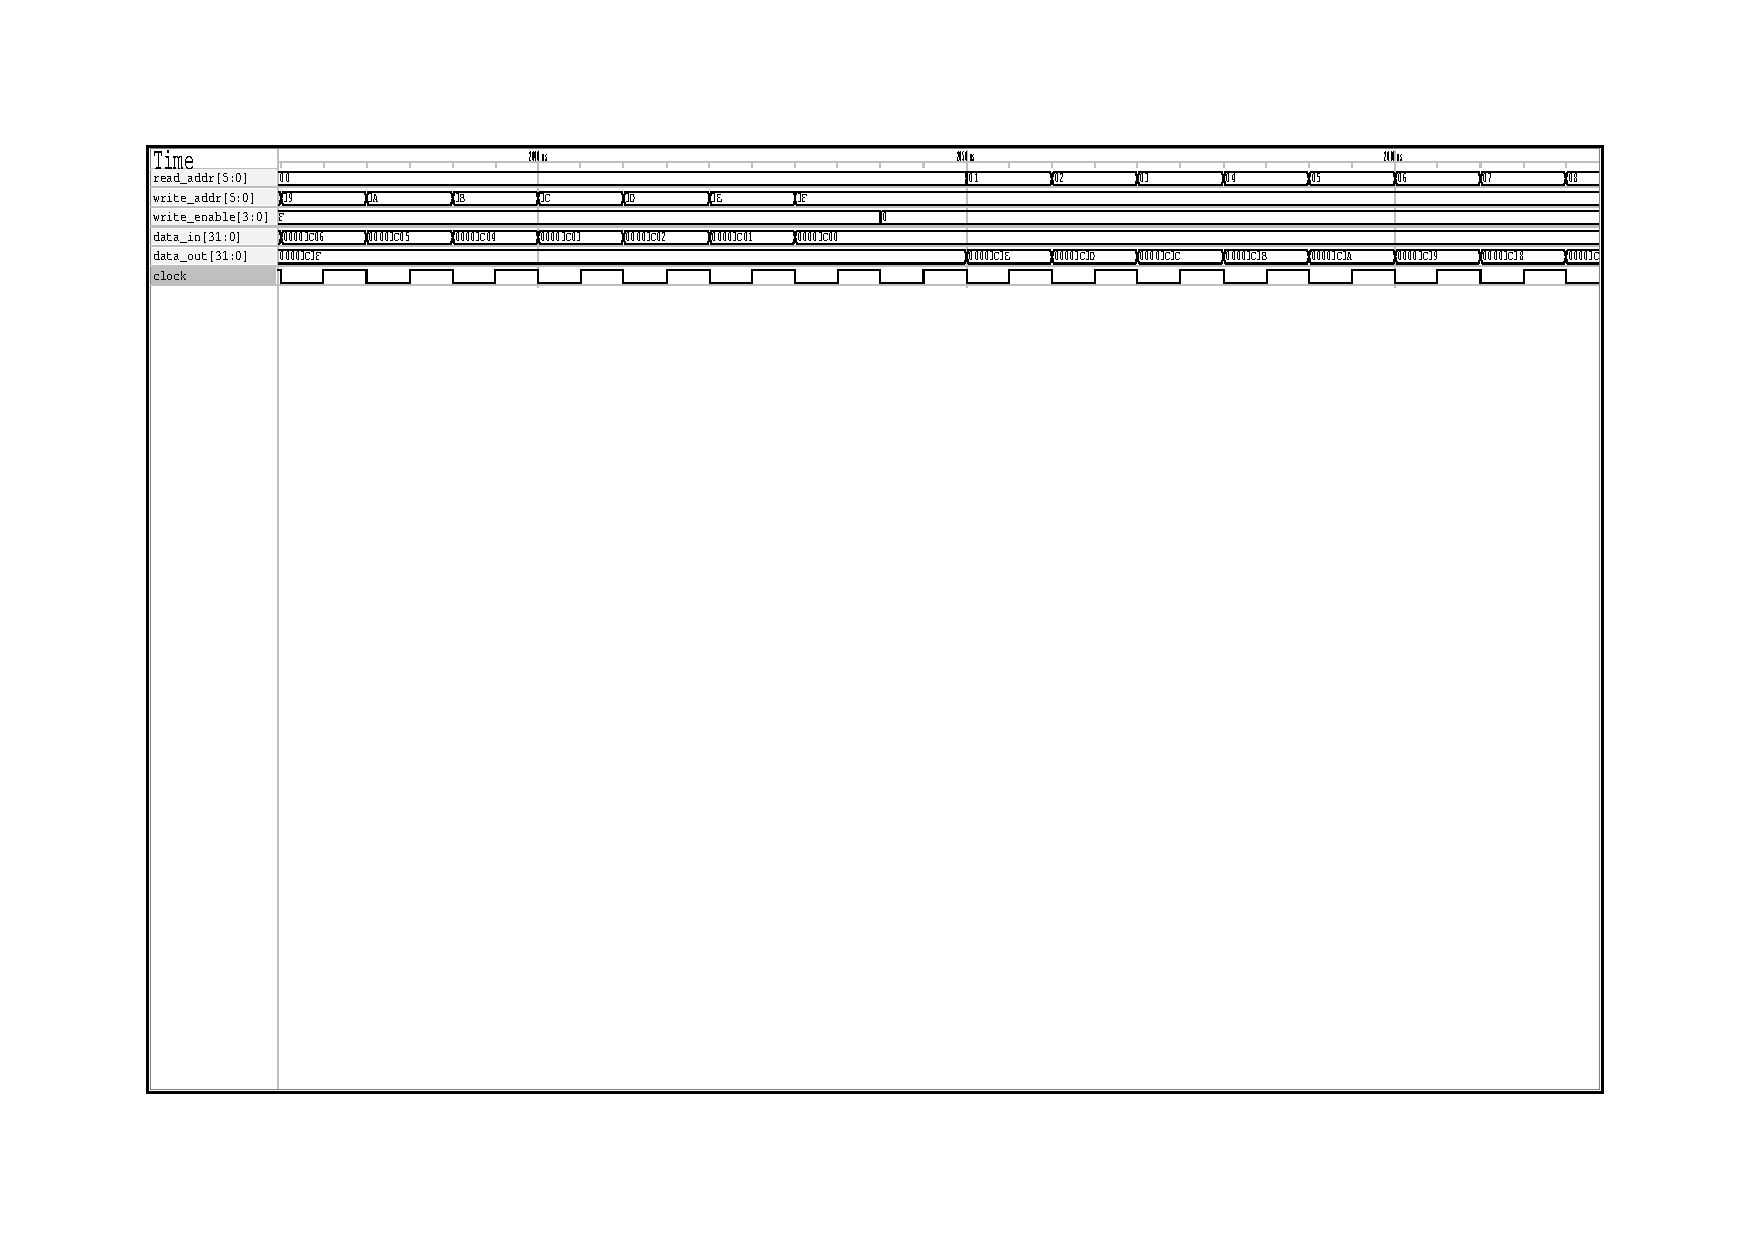
\includepdf[landscape=true]{../output/data_memory_tb.pdf}
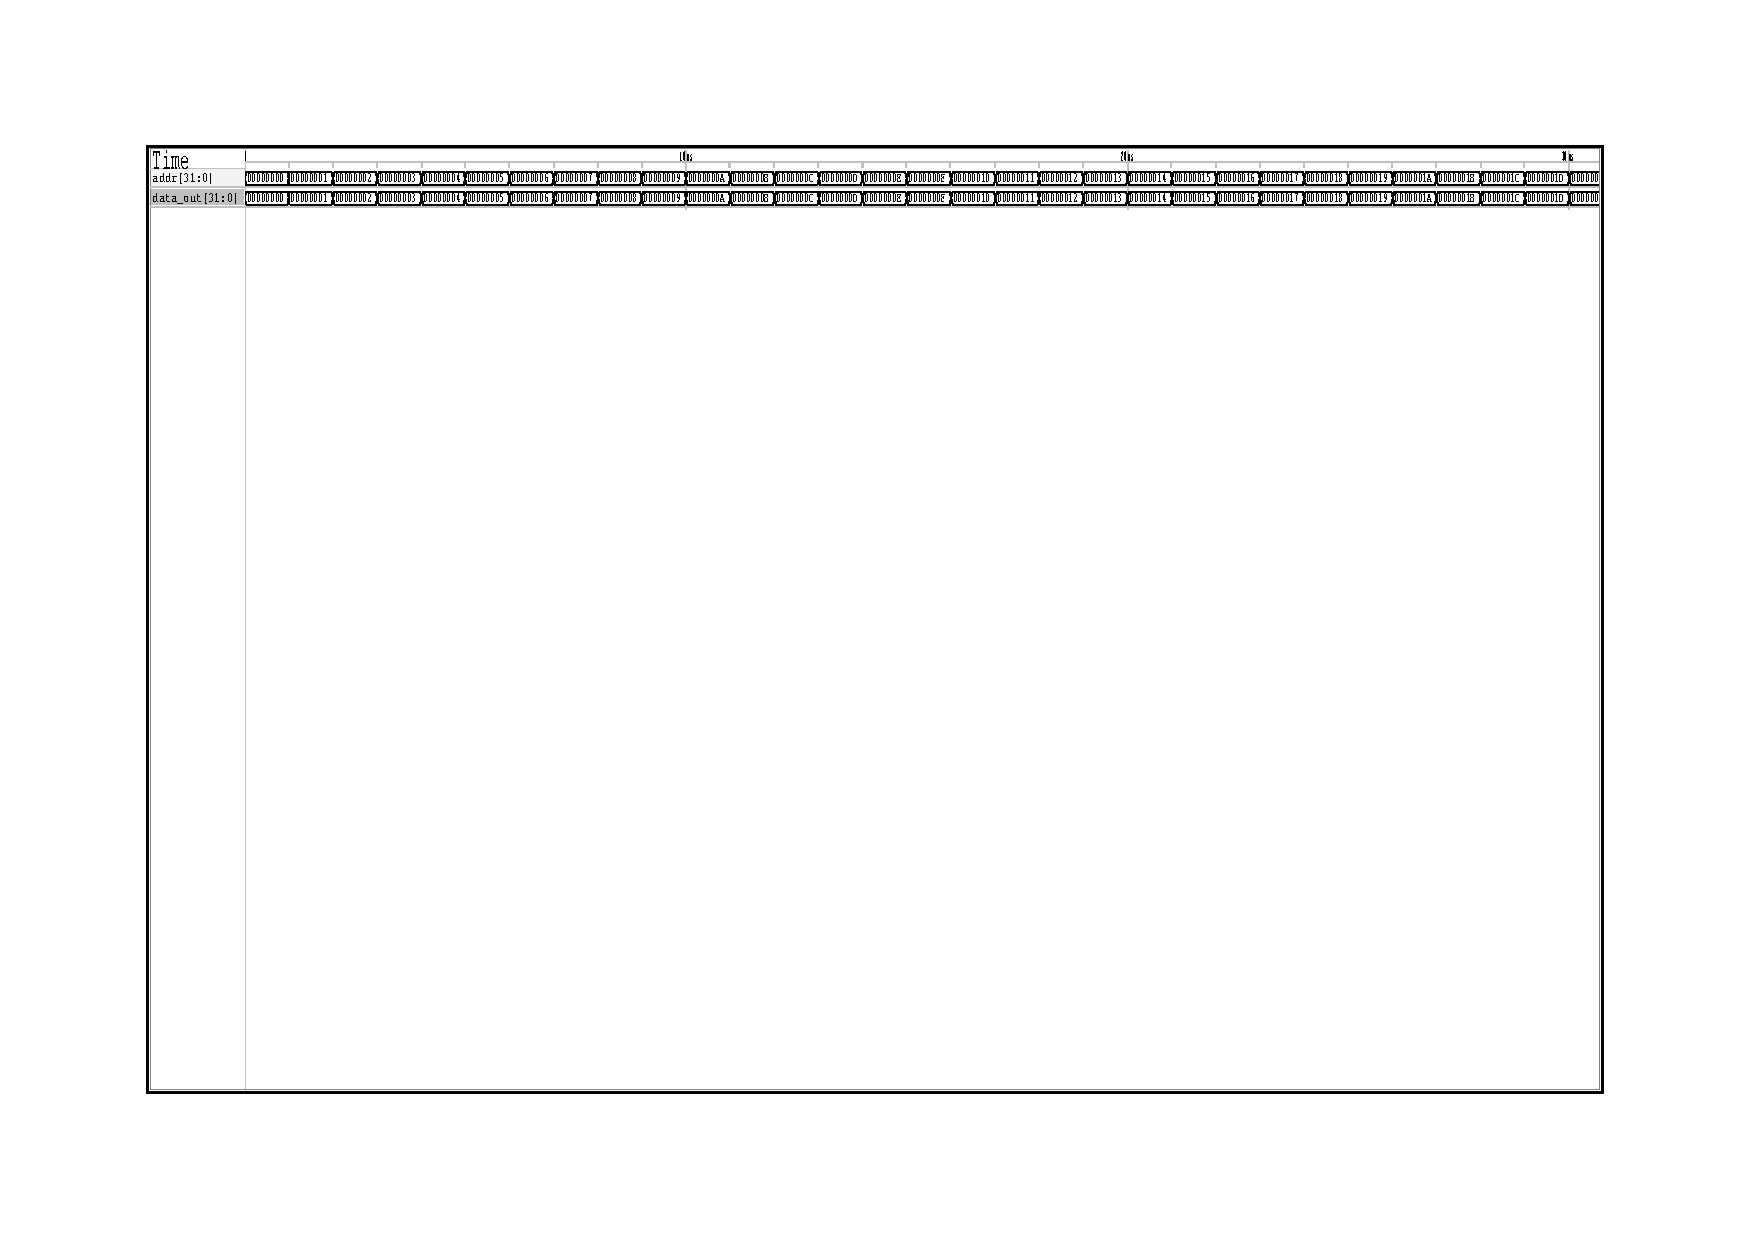
\includepdf[landscape=true]{../output/primary_memory_tb.pdf}
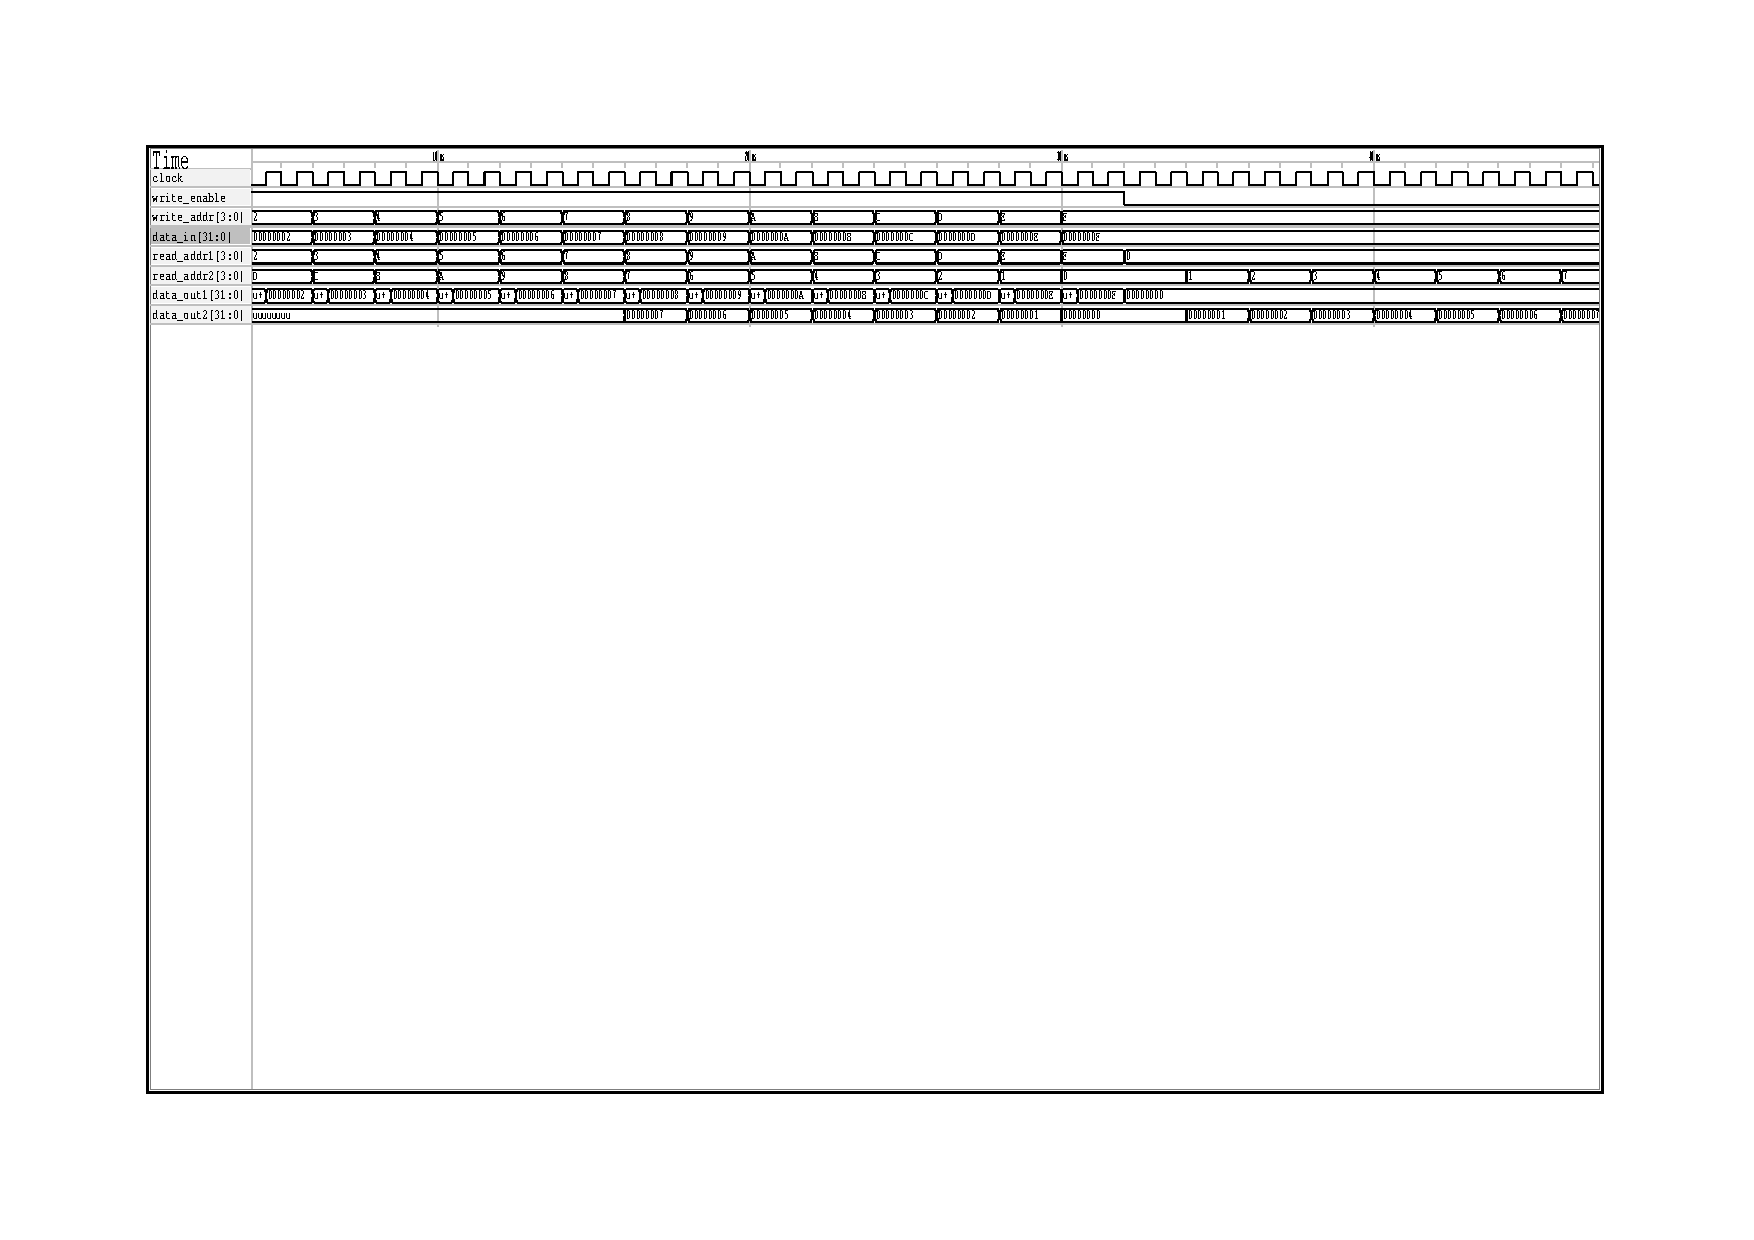
\includepdf[landscape=true]{../output/reg_file_tb.pdf}
\end{document}
